\section{Case Study of Ebola Related Rumor}
Mark Twain is credited with saying that a lie can travel halfway around the world while the truth is putting on its shoes. As the Ebola disease rages on in West Africa, the only other epidemic being talked about is the rapid spread of misinformation on social media about the disease, its origins and impact, and response strategies. We sought to characterize the spread of both news and rumors on Twitter about the deadly disease with a view to understanding the prevalence of misinformation.

For context, although Ebola is not a new disease, the current outbreak happening in West Africa is believed to be more than three times worse than all the previous Ebola outbreaks in history combined. The three countries that have the most widespread transmission, viz. Guinea, Liberia, and Sierra Leone, are also those where public health experts fear massive under-reporting due to a variety of social considerations. Even syndromic surveillance strategies, e.g., social media mining and participatory surveillance, are not effective in these countries due to poor penetration of Internet use, and lack of roads and communication infrastructure where Ebola is most prevalent.

Social media has become one of the primary sources by which people learn about worldwide developments so it is instructive to study the spread of Ebola related information on Twitter. Most of the current chatter on Twitter about Ebola reached its peak during late Sep-mid Oct (2014) during which period there have been Ebola-related developments in the US and Europe. (In contrast, Twitter penetration in the three specific West African countries is low.)

A brief timeline of these developments will help in the discussion that follows. On September 30, 2014, the CDC confirmed the first importation of Ebola into the United States when Thomas Eric Duncan traveled from Liberia to visit family in Dallas. On October 6, in Madrid, Spain, Teresa Romero, a nurse, was reported to be the first person to have contracted the disease outside of West Africa.

On October 8, back in the US, Duncan succumbed to Ebola. A few days later, a healthcare worker at Texas Presbyterian Hospital in Dallas who provided care for Duncan, tested positive for Ebola. On the morning of Oct. 14, a second healthcare worker, who also provided care for Duncan, reported to the hospital with a low-grade fever and was isolated. This healthcare worker also tested positive for Ebola subsequently.

Many states and cities began making contingency plans and issuing travel advisories and guidelines. Lawmakers called for screening passengers and proposed travel bans for Ebola-stricken countries. On October 23, Craig Spencer, a doctor returning from work in Guinea, was rushed to Bellevue Hospital Center with a 100.3 fever and became New York City�s first Ebola patient.


\subsection{Rumors on Twitter}
\begin{figure}[h]
\centering
\subfigure[09/29/14]{
   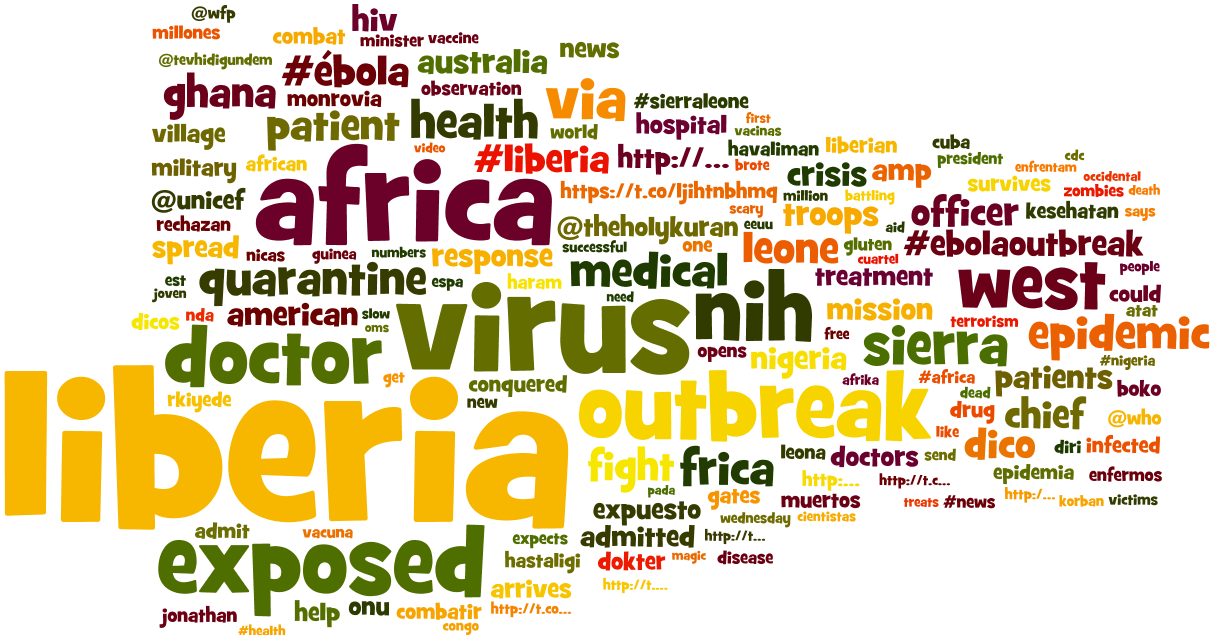
\includegraphics[width=2in,height=1.1in] {pictures/Ebola/Word_cloud_0929.png}
  \label{fig:worldcloud29}
 }
 \subfigure[09/30/14]{
   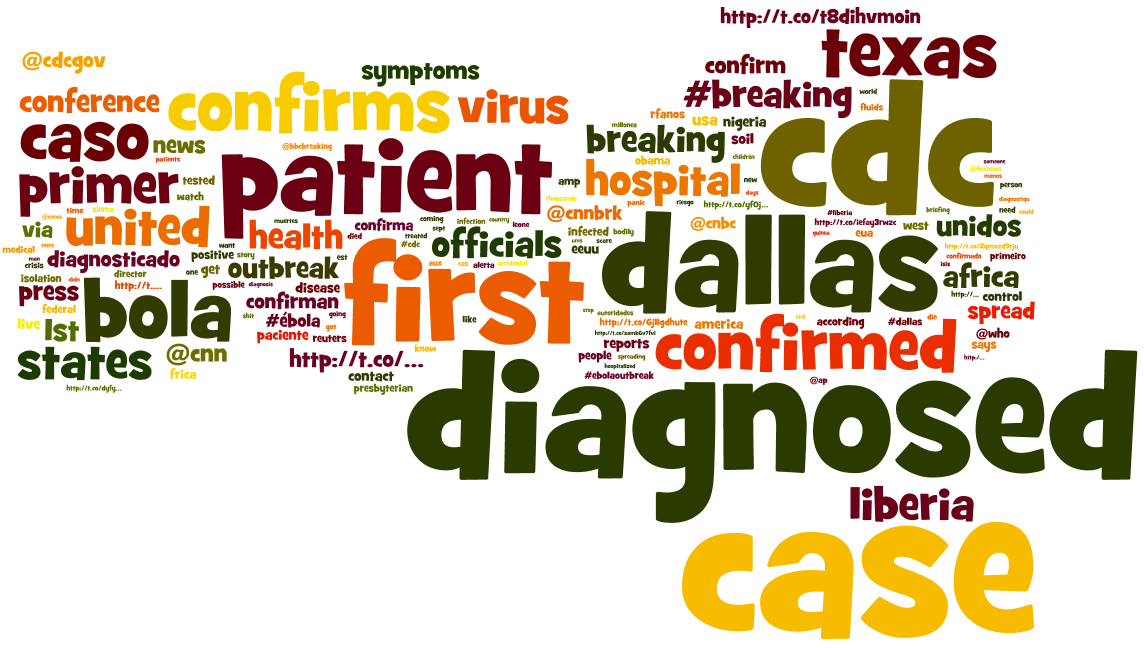
\includegraphics[width=2in,height=1.1in] {pictures/Ebola/Word_cloud_0930.png}
  \label{fig:worldcloud30}
 }
 \subfigure[10/01/14]{
   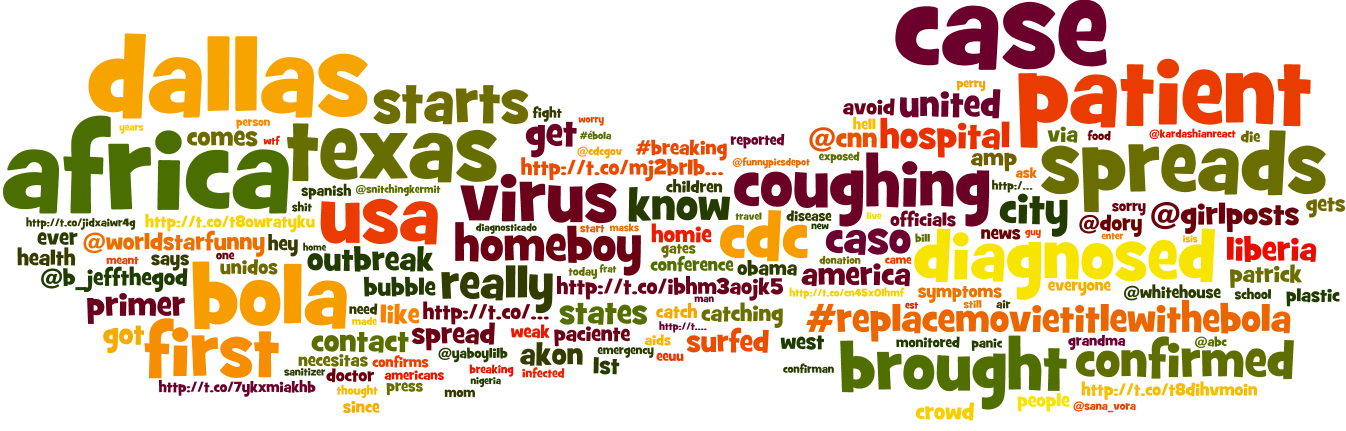
\includegraphics[width=2in,height=1.1in] {pictures/Ebola/Word_cloud_1001.png}
  \label{fig:worldcloud01}
 }
\caption{Word clouds constructed from Ebola-related tweets.}
\label{fig:Ebola_word_cloud}
\end{figure}

The period from end of Sep to mid-late Oct, when Ebola activity happened in the US, is also the period when conspiracy theories, innuendo and rumors began to propagate wildly on Twitter. We gathered tweets during this period and filtered them by either the mention of the keyword `ebola' or relevant hashtags such as \#ebola, \#EbolaVirus, \#EbolaOutbreak, \#EbolaWatch, \#EbolaEthics, \#EbolaChat, \#nursesfightebola, \#ebolafacts, \#StopEbola, \#FightingEbola, and \#UHCRevolution.

From the gathered tweets, we removed stopwords for further processing. Figure~\ref{fig:Ebola_word_cloud} depicts word clouds constructed from the tweets for specific days. As can be seen, on 2014-09-29, when there was no Ebola incident in the US, people�s attention were primarily focused on Liberia and other African countries. On 2014-09-30, after CDC confirmed that Mr. Duncan in Dallas tested positive for Ebola, related keywords rose to the fore.


%Figure~\ref{fig:Ebola_time_series} depicts a simple frequency plot of specific keywords in Ebola-related tweets highlighting significant upticks for keywords such as Dallas, USA, CDC as well as �enfermera� (referring to the Spanish Nurse Romero and possibly other health professionals) during the studied period. Into mid October, we notice upticks in mentions of President Obama, likely due to proposed mitigation and response strategies by the US Government.
%
%
%\begin{figure}[ht]
%\centering
%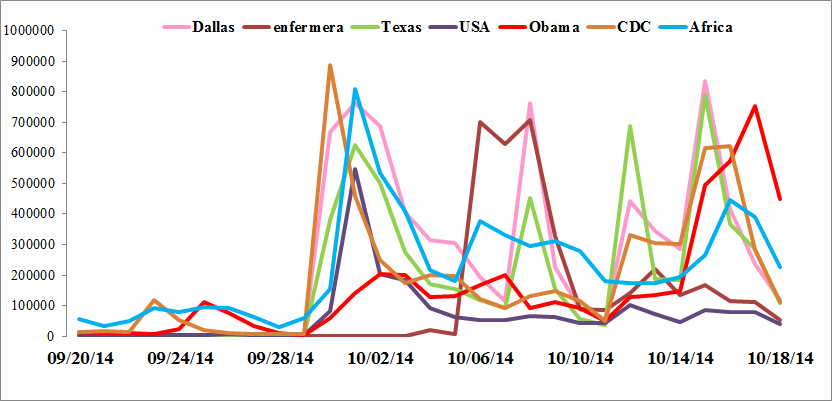
\includegraphics[width=5in]{pictures/time_series.png} %?????????????
%\caption{Frequency plot of specific keywords in Ebola-related tweets from 09/20/2014 to 10/18/2014}
%\label{fig:Ebola_time_series}
%\end{figure}

\begin{figure}[h]
\centering
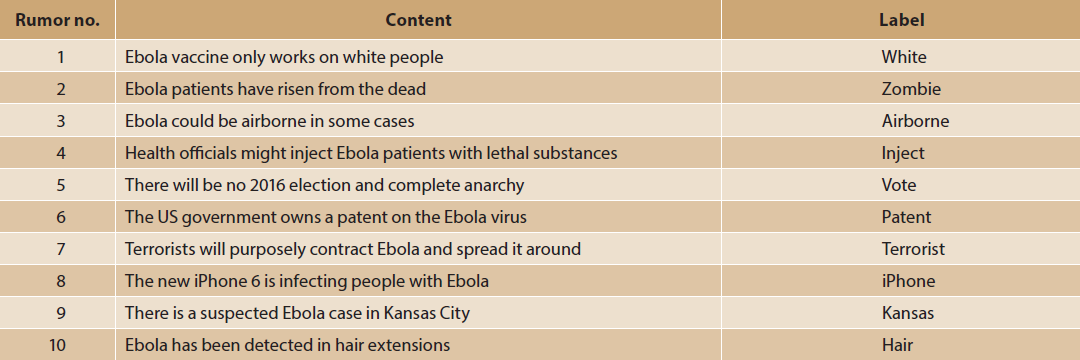
\includegraphics[width=6.5in, height=2.3in]{pictures/Ebola/10_rumors_1.png} %?????????????
\caption{Top 10 Ebola-related rumors (by volume; from 09/28/2014 to 10/18/2014).}
\label{fig:Ebola_10rumors}
\end{figure}

\begin{figure}[h]
\centering
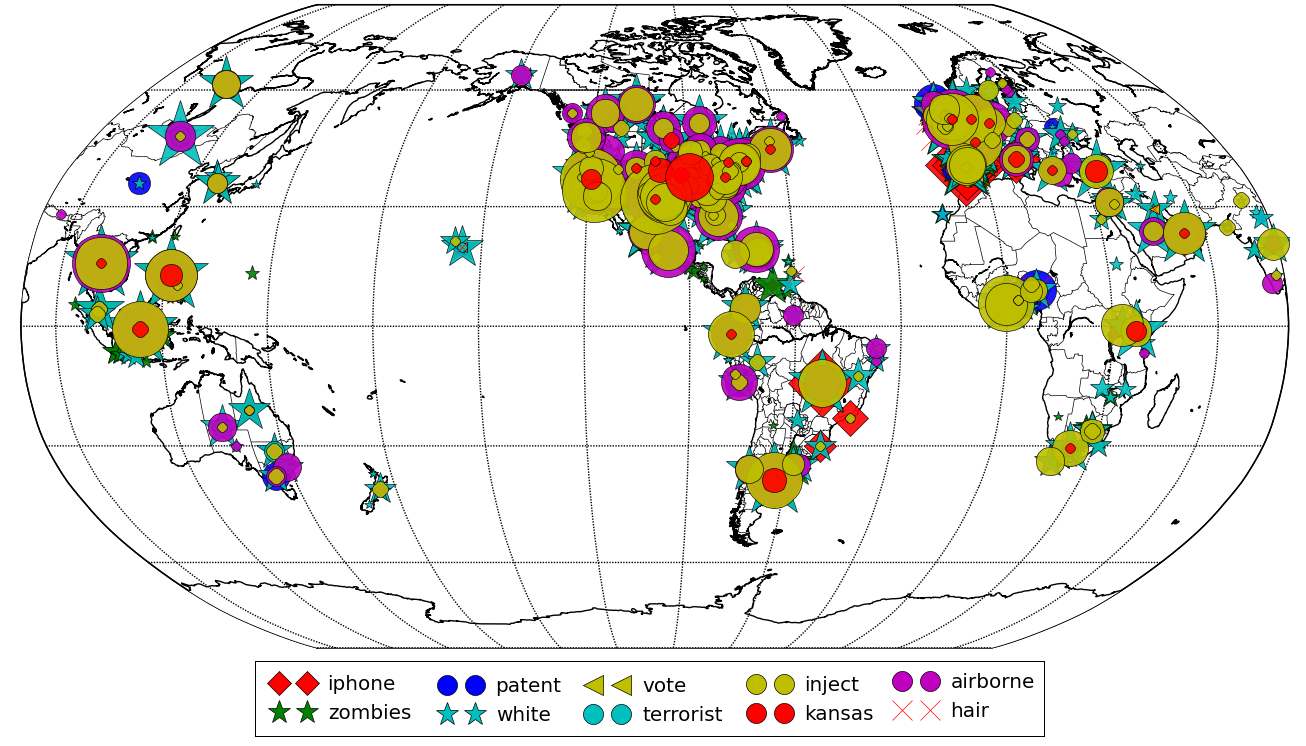
\includegraphics[width=5in]{pictures/Ebola/20141008-map-country1.png} %?????????????
\caption{Distribution of top-10 rumors obtained from geolocated tweets. Data from 10/08/2014 is used for this plot. Icon size is proportional to the logarithm of the tweet volume.}
\label{fig:Ebola_map}
\end{figure}


Next, we studied information cascades in our collection of tweets with a view toward identifying misinformation and spread of falsehoods. We identified several widespread rumors circulating on Twitter, the top 10 of which are shown in Figure~\ref{fig:Ebola_10rumors}. (We focus on rumors in English only for our study.) Most are self-explanatory as to their intent and interpretation.


Two other rumors are note worthy. The `snake' rumor (which originated at least as early as late summer 2014) asserts that Ebola came across the border from Guinea to Sierra Leone via a snake in a bag. As stated in [4], ``a lady had a snake in a bag. When somebody opened the bag, that made the lady die.'' The Maldives rumor pertains to an uncorroborated report that Ebola patients have been reported (and quarantined) in the Maldives.

For each of these rumors, we geocoded tweets participating in the spread of such rumors with a view to understanding their geographical scope. As Figure~\ref{fig:Ebola_map} shows, the ``airborne'' and ``inject'' rumors were most prevalent in the US with specific other rumors (e.g., ``patent'') being prevalent in other parts of the world.



\begin{figure}[h]
\centering
\subfigure[09-29-2014]{
   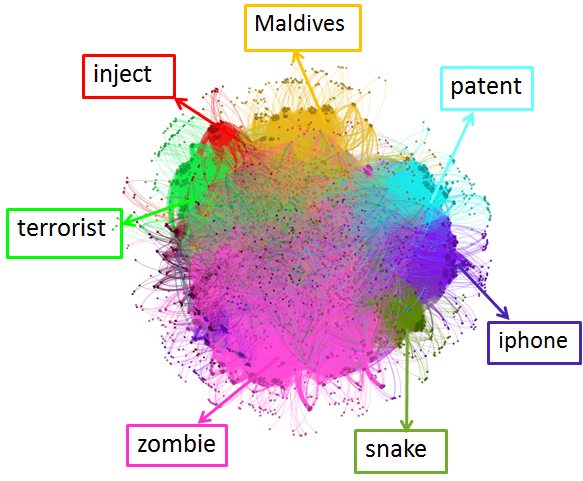
\includegraphics[width=3in] {pictures/Ebola/rumor-cluster-20140929.png}
  \label{fig:worldcloud29}
 }
 \subfigure[10-06-2014]{
   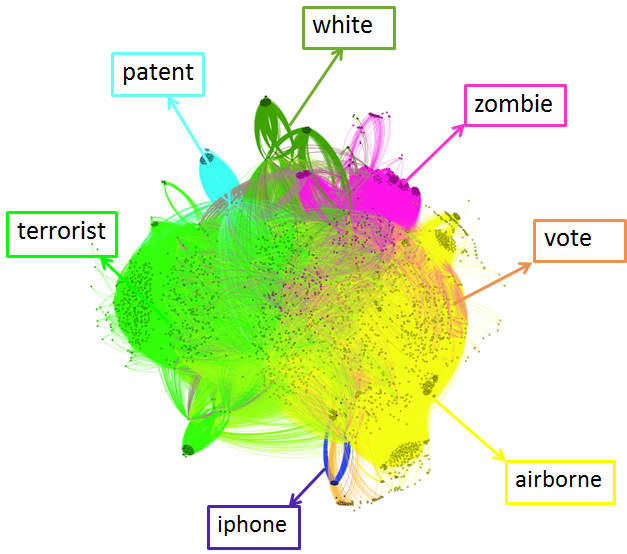
\includegraphics[width=3in] {pictures/Ebola/rumor-cluster-20141006.png}
  \label{fig:worldcloud30}
 }
\caption{How rumors cluster: (a) 09/29/2014. (b) 10/06/2014. Rumors are color coded consistently across the two frames.}
\label{fig:Ebola_cluster}
\end{figure}

Next, we employed a dynamic query expansion model~\cite{zhao2014unsupervised} to study the rumors in greater detail. The DQE model begins with a seed set of keywords (e.g., ``ebola'', ``rumor''), identifies tweets that mentions these keywords, and iteratively expands them into a larger set of keywords. By conducting a modularity-based optimization over the underlying network of expanded tweets connected by shared keywords, DQE can identify specific localized instantiations of rumors.

As shown in Figure~\ref{fig:Ebola_cluster}, on 09/29/2014 (when there was no incidence of Ebola in the US), the dominant rumor is the zombie rumor. By 10/06/2014, other rumors pertaining to how Ebola can be airborne and that it is a potential terrorist weapon gained hold.



Although Figure~\ref{fig:Ebola_cluster} might suggest that rumors are quite rampant, it is important to keep in perspective that they are but a small fraction of all information propagation related to Twitter. Figure~\ref{fig:Ebola_patent_propagation} and~\ref{fig:Ebola_news_propagation} compare the time-indexed spread of the `patent' rumor versus a true news story (about the first US incidence of Ebola in Dallas). Here different colors denote different communities participating in information propagation, not different rumors/news stories. Each node in these graphs denotes a Twitter user, and an edge between nodes denotes a reply or retweet relationship. As can be seen, news stories permeate better whereas rumors are more localized, distributed, and comparatively smaller in permeation.

\begin{figure}[h]
\centering
\subfigure[09-30-2014]{
   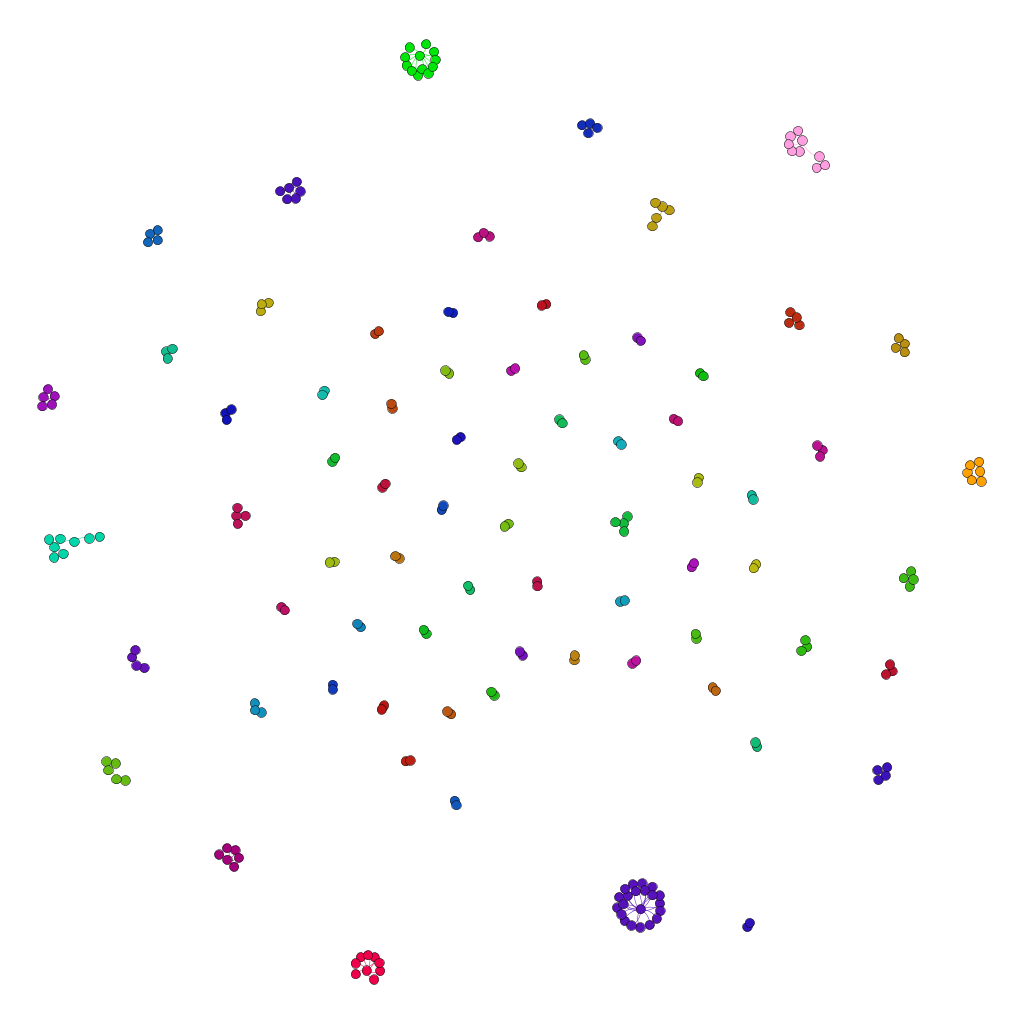
\includegraphics[width=2in] {pictures/Ebola/patent_20140930.png}
  \label{fig:patent_20140930}
 }
 \subfigure[09-30-2014]{
   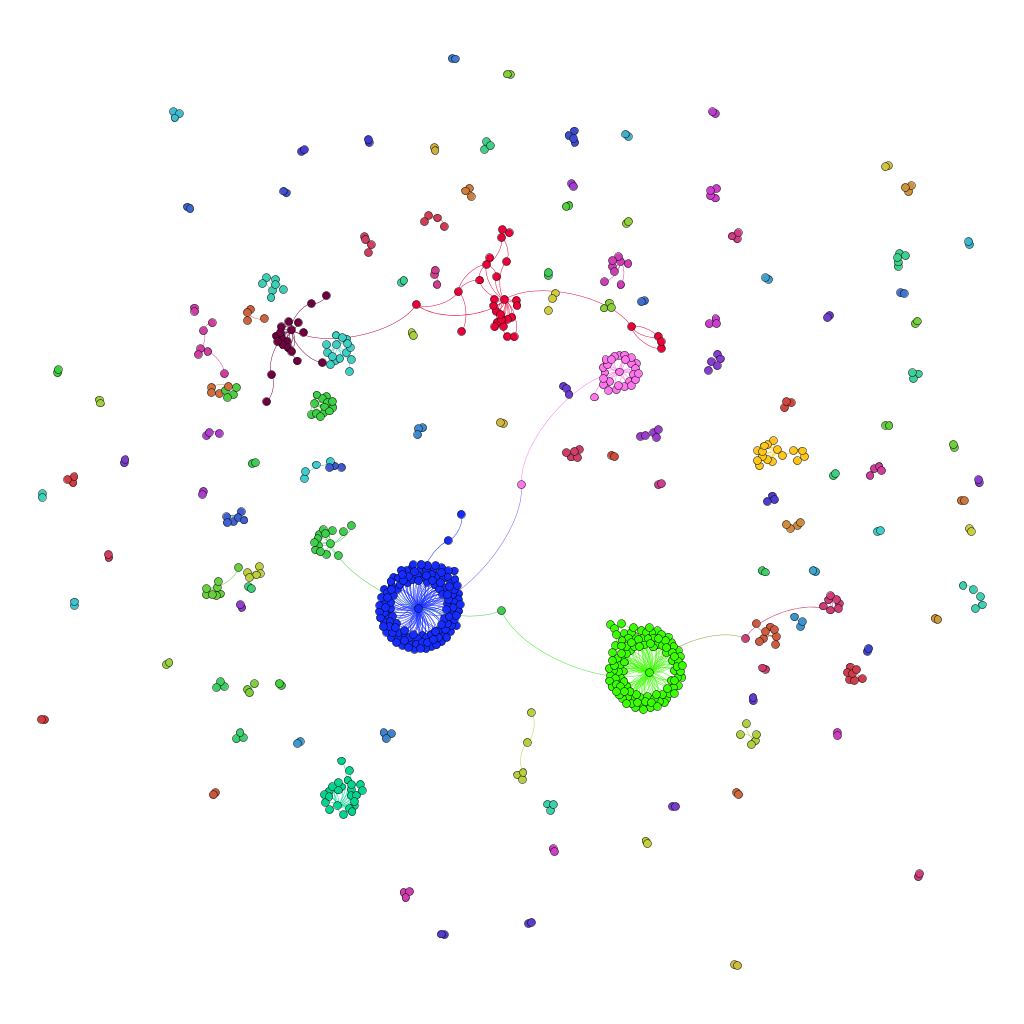
\includegraphics[width=2in] {pictures/Ebola/patent_20141001.png}
  \label{fig:patent_20141001}
 }
 \subfigure[10-01-2014]{
   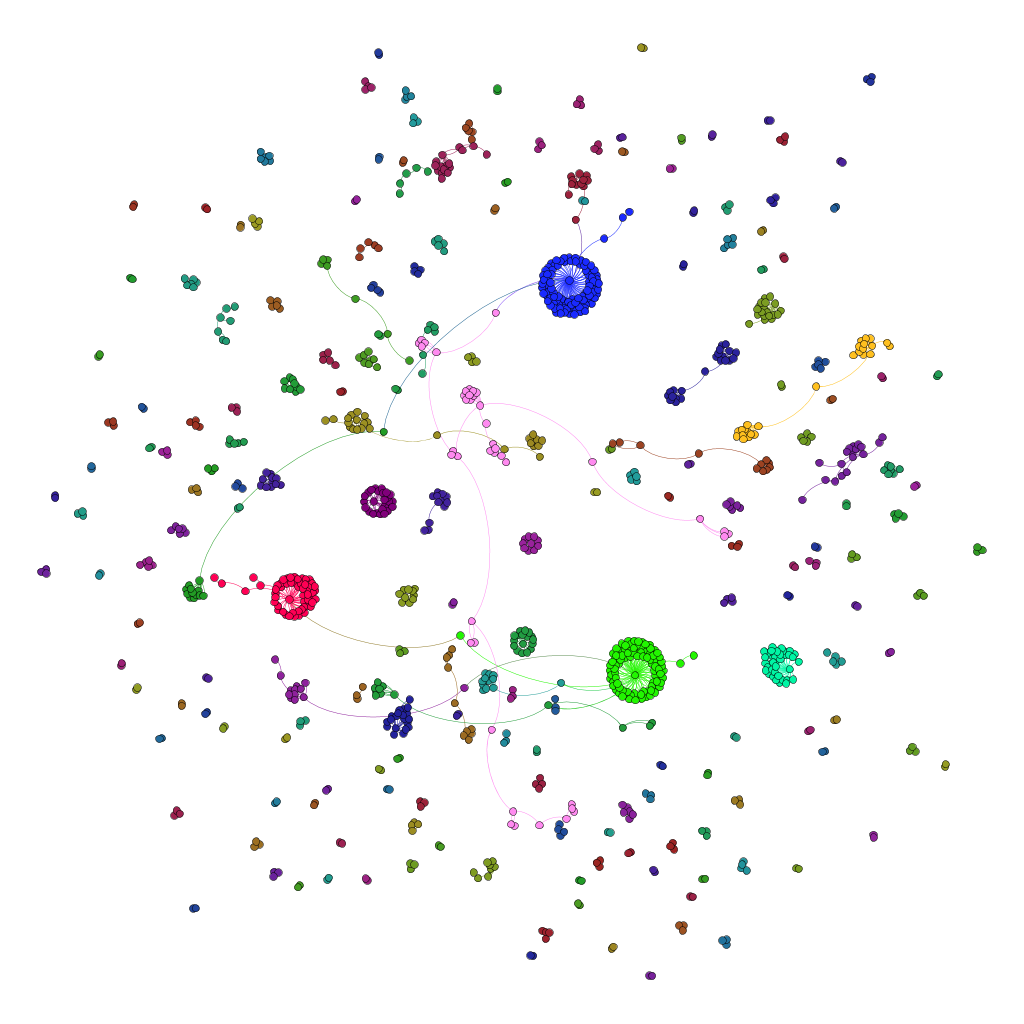
\includegraphics[width=2in] {pictures/Ebola/patent_20141002.png}
  \label{fig:patent_20141002}
 }
\caption{Ebola-related patent rumor propagation over time.}
\label{fig:Ebola_patent_propagation}
\end{figure}



\begin{figure}[h]
\centering
\subfigure[09-30-2014]{
   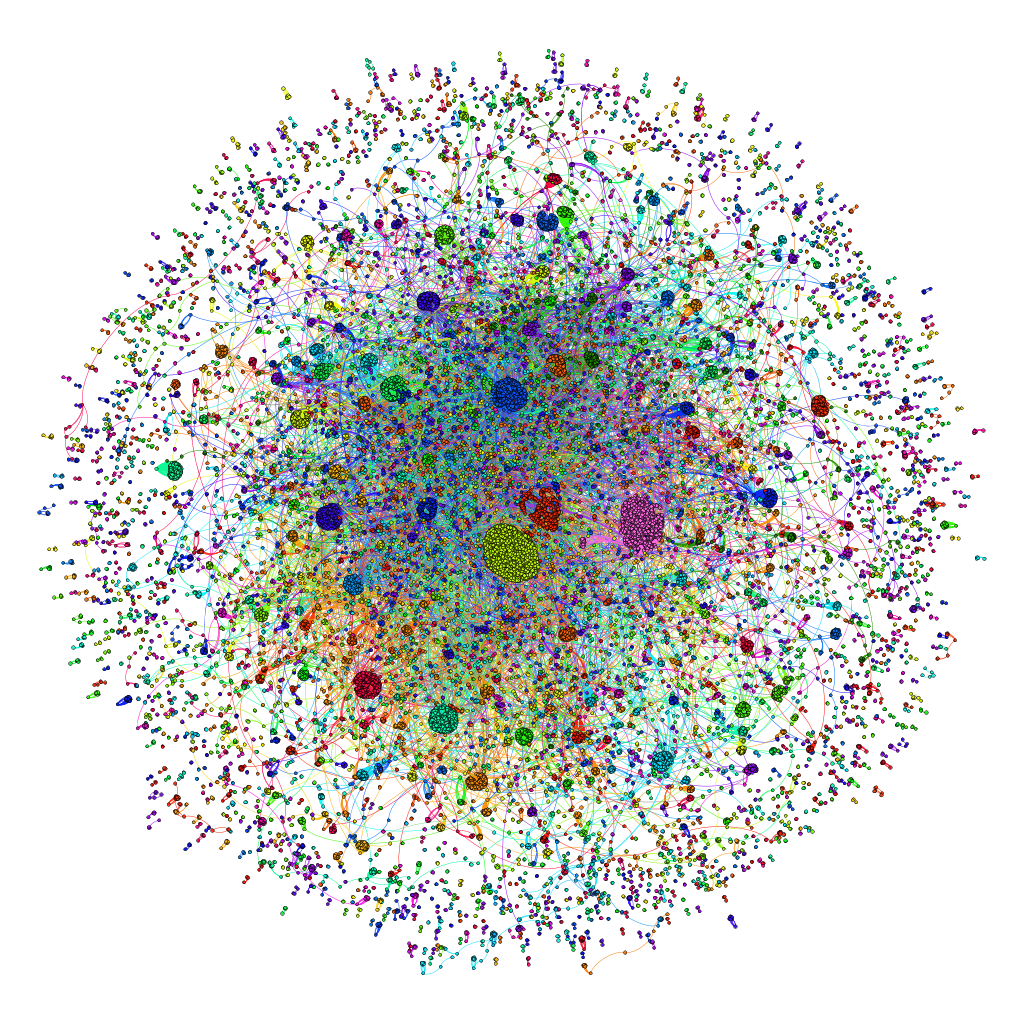
\includegraphics[width=2in] {pictures/Ebola/dallas_20140930.png}
  \label{fig:dallas_20140930}
 }
 \subfigure[09-30-2014]{
   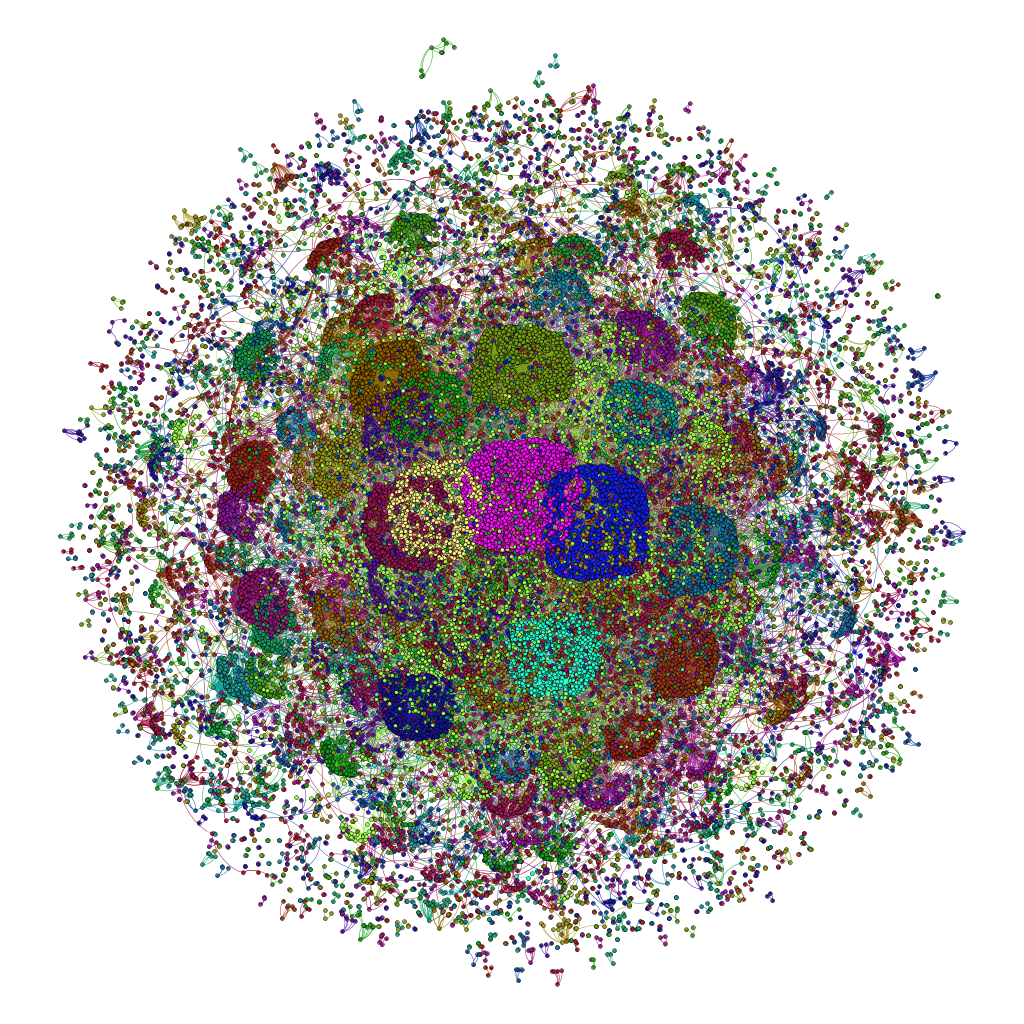
\includegraphics[width=2in] {pictures/Ebola/dallas_20141001.png}
  \label{fig:dallas_20141001}
 }
 \subfigure[10-01-2014]{
   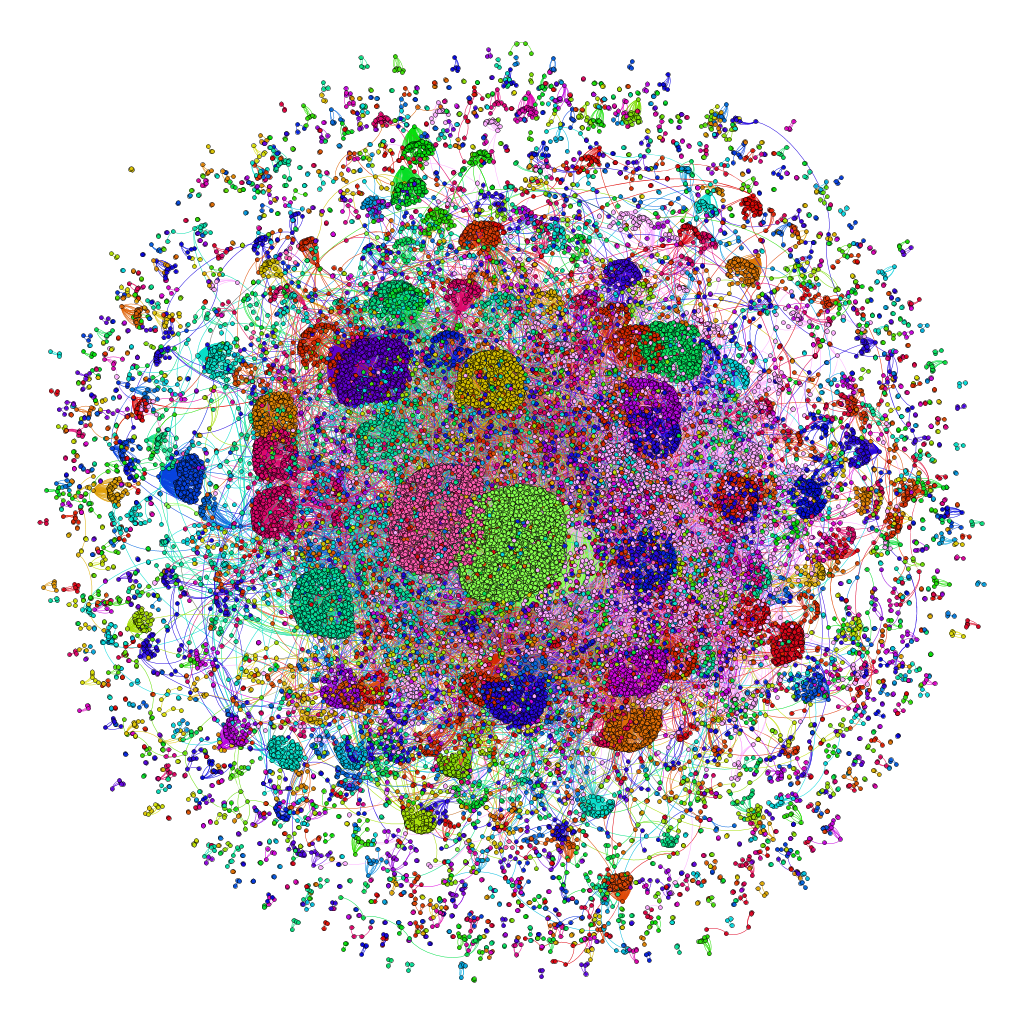
\includegraphics[width=2in] {pictures/Ebola/dallas_20141002.png}
  \label{fig:dallas_20141002}
 }
\caption{Ebola-related Dallas news propagation over time.}
\label{fig:Ebola_news_propagation}
\end{figure}


\subsection{Epidemiological Modeling of Rumors}
Another way to study the spread of rumors (versus news) is from an epidemiological modeling standpoint. An epidemiological model helps capture the likelihood of an individual getting infected with a virus or, here, of adopting an idea that he or she has been exposed to.

\begin{figure}[h]
\centering
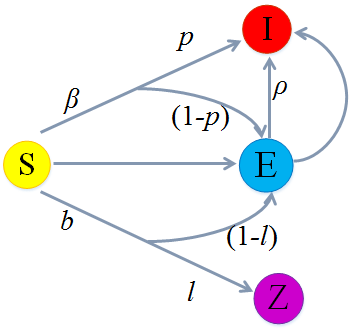
\includegraphics[width=2in]{pictures/Ebola/SEIZ.png} %?????????????
\caption{The SEIZ compartmental model. The various states denote: (S) Susceptible. (I) Infected. (E) Exposed. (Z) Skeptic.}
\label{fig:Ebola_SEIZ_raw}
\end{figure}


\begin{figure}[h]
\centering
\subfigure[white]{
   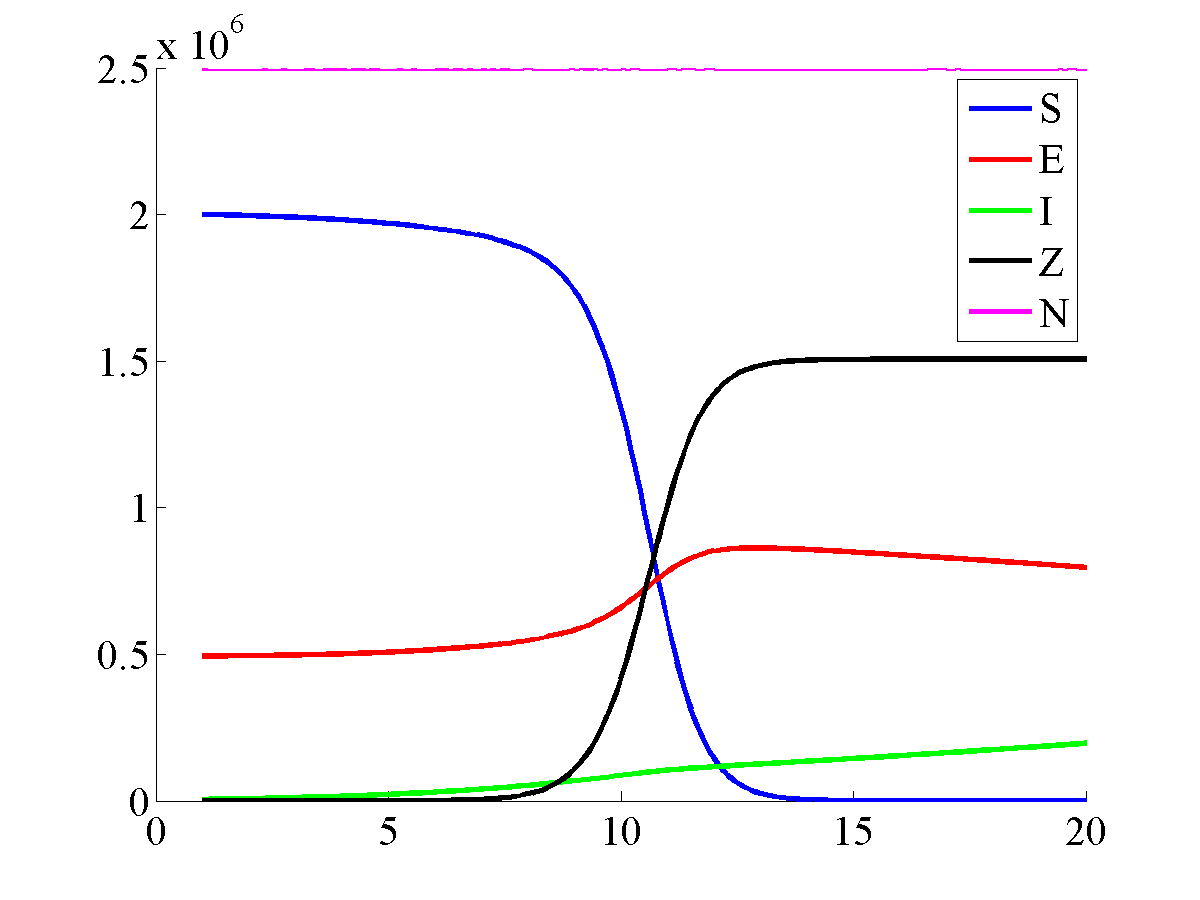
\includegraphics[width=1.45in] {pictures/Ebola/b-white_SEIZ_timecourse.png}
  \label{fig:b-white_SEIZ_timecourse}
 }
 \subfigure[zombies]{
   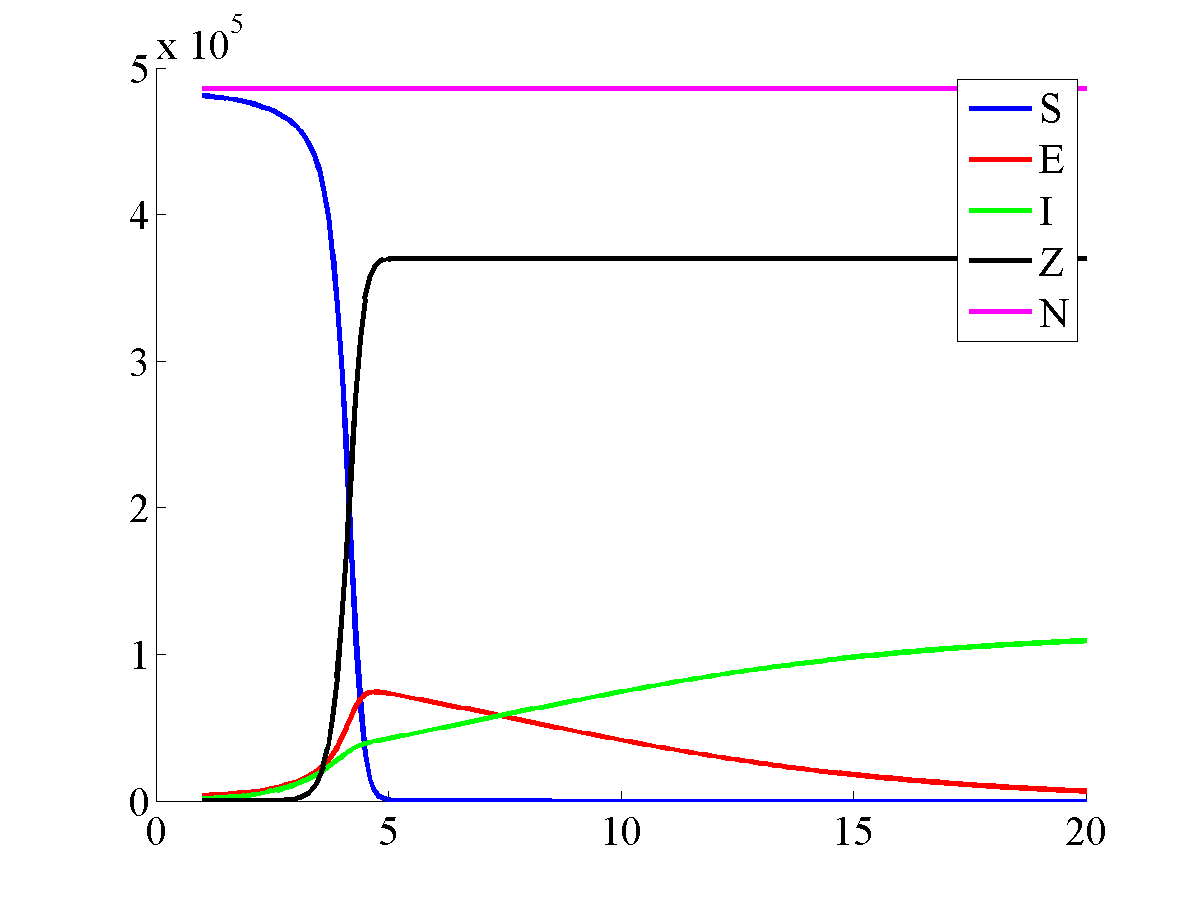
\includegraphics[width=1.45in] {pictures/Ebola/c-zombies_SEIZ_timecourse.png}
  \label{fig:c-zombies_SEIZ_timecourse}
 }
 \subfigure[airborne]{
   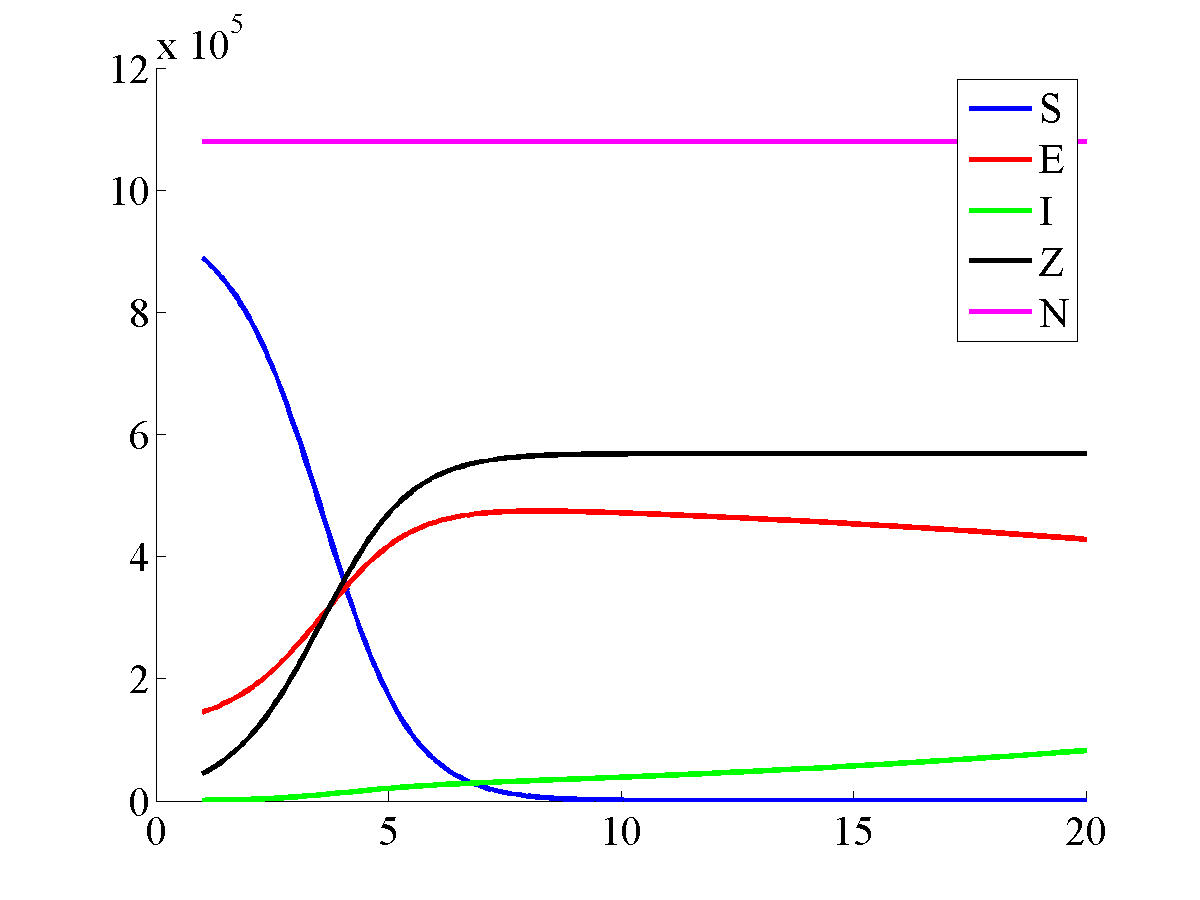
\includegraphics[width=1.45in] {pictures/Ebola/d-airborne_SEIZ_timecourse.png}
  \label{fig:d-airborne_SEIZ_timecourse}
 }
  \subfigure[patent]{
   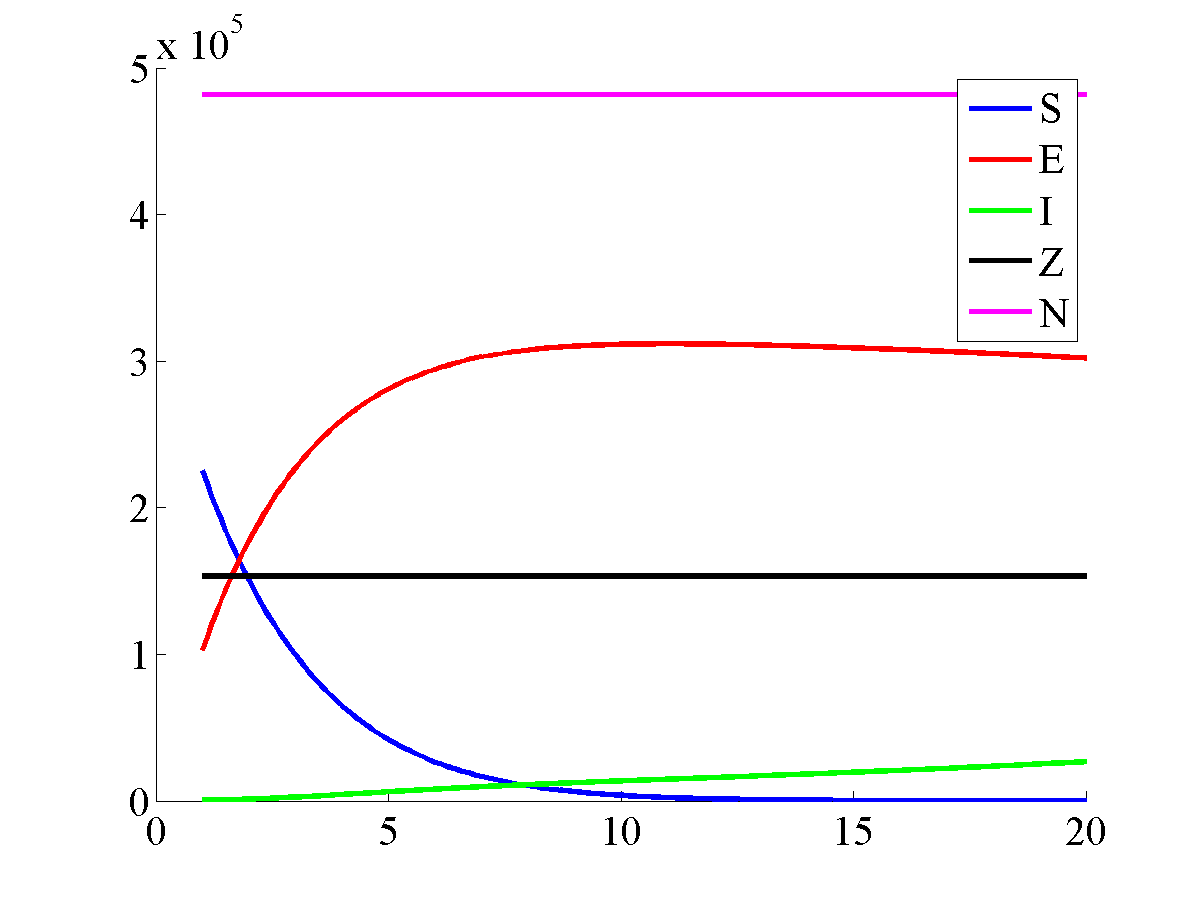
\includegraphics[width=1.45in] {pictures/Ebola/e-patent_SEIZ_timecourse.png}
  \label{fig:e-patent_SEIZ_timecourse}
 }
 \subfigure[white]{
   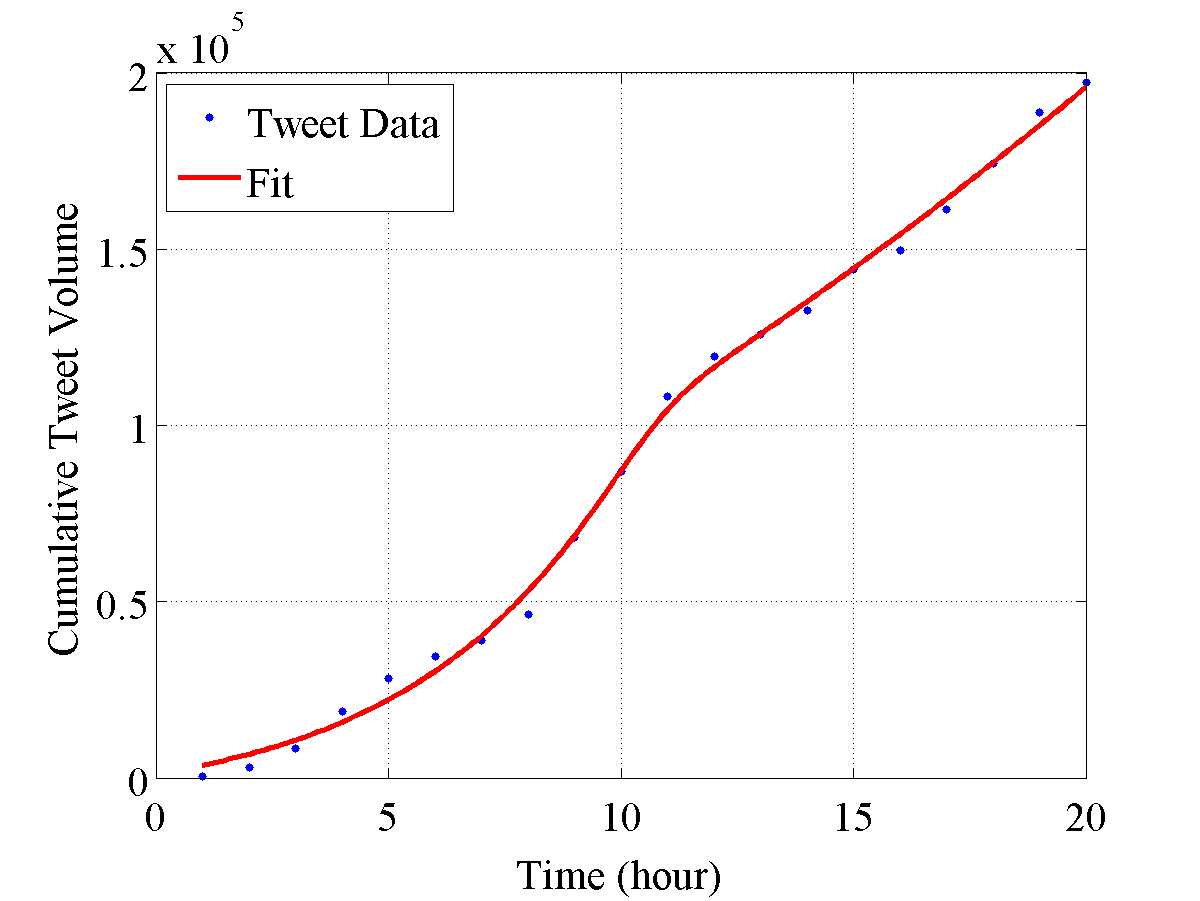
\includegraphics[width=1.45in] {pictures/Ebola/Fig7-white-fitting.png}
  \label{fig:Ebola-white-fitting}
 }
 \subfigure[zombies]{
   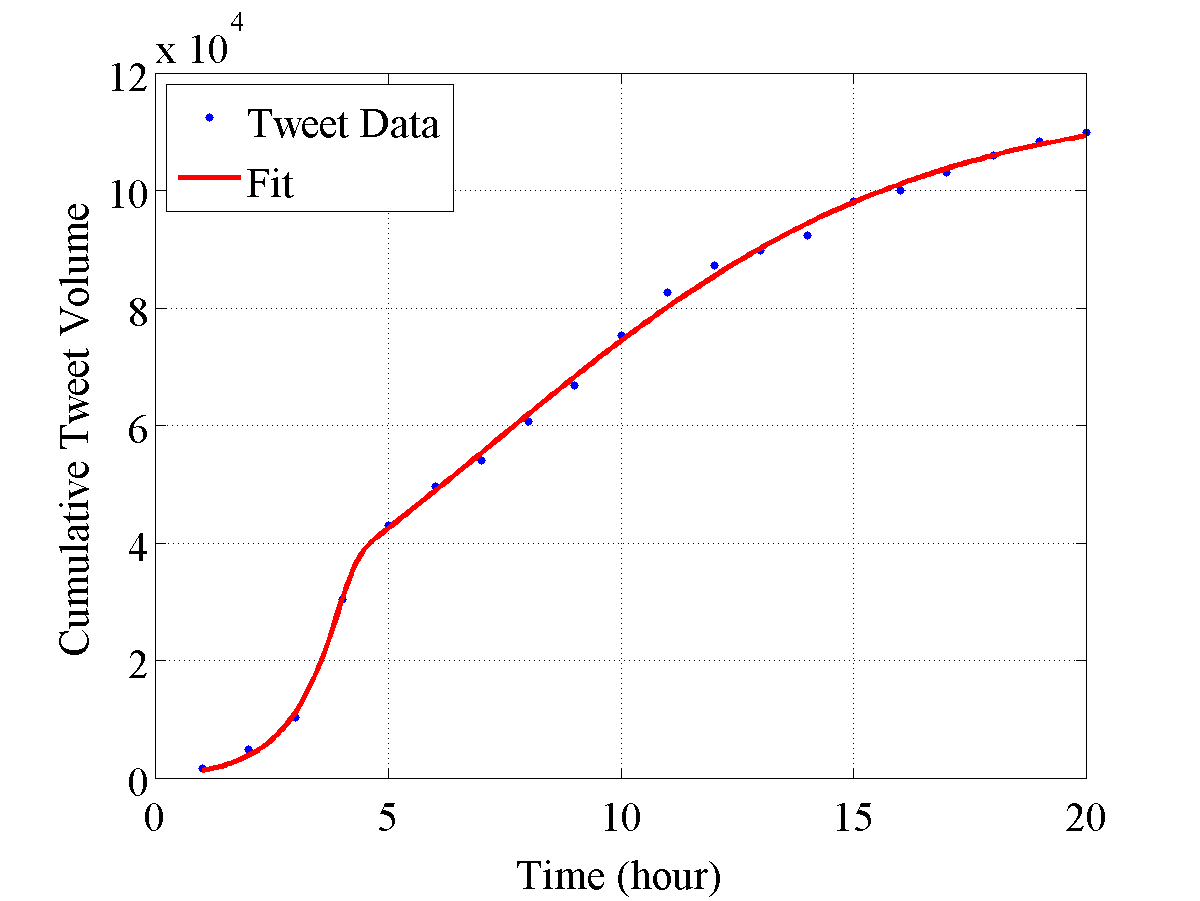
\includegraphics[width=1.45in] {pictures/Ebola/Fig7-zombies-fitting.png}
  \label{fig:Ebola-zombies-fitting}
 }
 \subfigure[airborne]{
   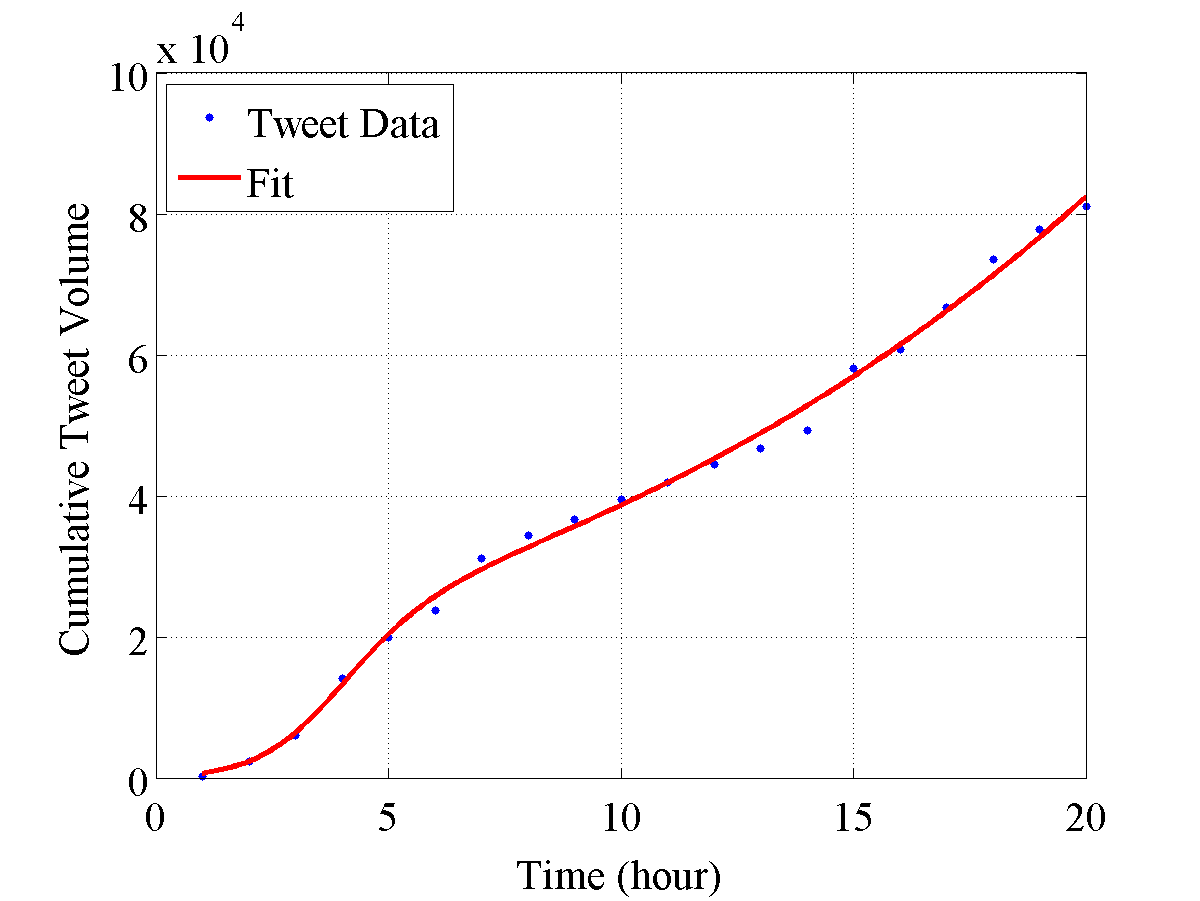
\includegraphics[width=1.45in] {pictures/Ebola/Fig7-airborne-fitting.png}
  \label{fig:Ebola-airborne-fitting}
 }
  \subfigure[patent]{
   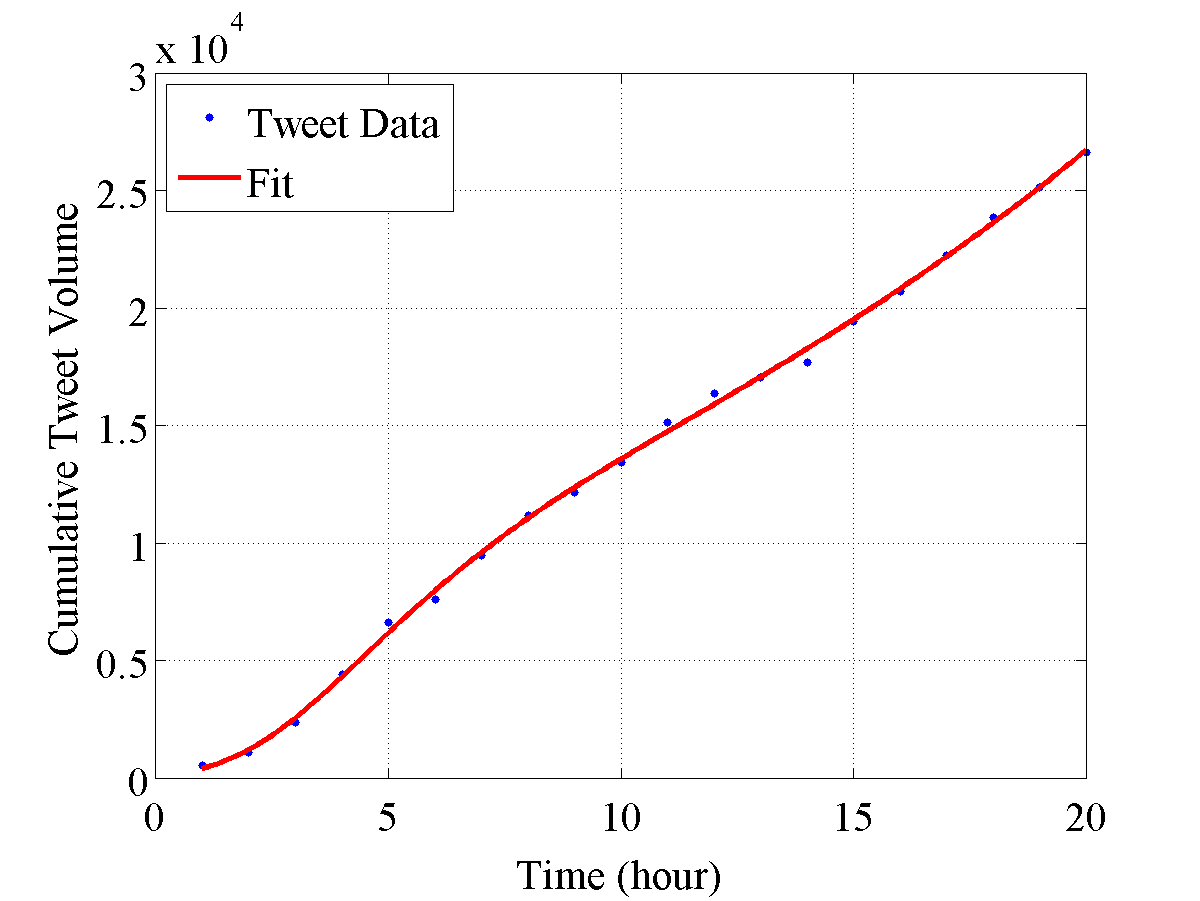
\includegraphics[width=1.48in] {pictures/Ebola/Fig7-patent-fitting.png}
  \label{fig:Ebola-patent-fitting}
 }
\caption{Model fits of SEIZ to different rumors: (from left to right) �white�, �zombies�, �airborne�, and �patent�. (top row) Fitting results. (bottom row) time-course profiles of different compartments. }
\label{fig:Ebola_SEIZ_fitting}
\end{figure}

In earlier work~\cite{jin2013epidemiological} we demonstrated how we can accomplish this objective using the SEIZ epidemiological model that was originally proposed to study the adoption of ideas~\cite{powerofgoodidea:2006}. The SEIZ model is particularly suited to studying rumor propagation as it captures distinctions in how people respond to ideas: whether they adopt it readily or are initially skeptical.

The idea in the SEIZ model is to compartmentalize a population into four categories, denoted as S, E, I, and Z. We interpret these categories with specific reference to Twitter propagation. Susceptible (S) represents a user who has not heard the information; infected (I) denotes a user who has (re)tweeted about the information; skeptic (Z) denotes a user who has heard about the information but chooses not to (re)tweet about it; and exposed (E) represents a user who has received the information via a tweet but has taken some time, an exposure delay, prior to reposting or sharing that information.


The transitions between these states are modeled as shown in Fig~\ref{fig:Ebola_SEIZ_raw}. We caution that referring to the Z compartment as a �skeptic� is in no way an implication of the underlying truth or falsehood of the information; it simply helps capture whether users readily adopt an idea or take some time to adopt it.

Model fits of SEIZ to the different rumors and time course information for each of the state variables is given in Figure~\ref{fig:Ebola_SEIZ_fitting}. As can be seen the SEIZ model is capable of capturing a variety of information spread patterns: quasi-linear (e.g., �patent�), sigmoidal (�white�), and other non-linear patterns (�zombies� and �airborne�).


Time course results from the SEIZ compartmental model as shown in Figure~\ref{fig:Ebola_SEIZ_fitting} depict broadly similar patterns. Here �N� denotes the total size of the population (distinct Twitter users). High values of S rapidly decrease with a relatively comparable increase in Z, and a gradual increase in I that continues as E decreases. However, the patent rumor time-course data has a noticeably different response profile than the other rumor examples.

Here, the initial value of the S group begins with less than half of the total population size, and only slightly higher than the initial values of the Z and E groups. Second, the Z group is essentially constant, meaning that the number of skeptics does not change throughout the propagation time course. Third, the decrease in S does not correspond to a change in Z, as is observed in the other rumor examples. Rather, the drop in S is met with a near identical increase in E.


These findings hint that a large influx into E without a corresponding efflux to I combined with a stagnant Z group will produce an elevated response ratio. In other words, there is a large exposure to the rumor topic without significant change in skepticism.

In our earlier work on characterizing rumors~\cite{jin2013epidemiological}, we defined the notion of a �response ratio� which quantifies transitions through the exposed compartment. The response ratio provides a relative measure of the population influx into the E compartment versus the efflux from this compartment. We hypothesize that this ratio could be one of the factors useful in discriminating rumors from true news, with larger response ratios associated with factual news topics.

To compare response ratios across rumor and news, we select three breaking (true) news stories pertaining to Ebola: `Dallas' refers to the story of the first Ebola patient (Duncan) identified in the US; `NYC' refers to the first confirmation of an Ebola patient (Spencer) in New York City; and `Spencer' refers to the specific symptoms and travel activities of Spencer in the days before he was diagnosed.

\begin{figure}[h]
\centering
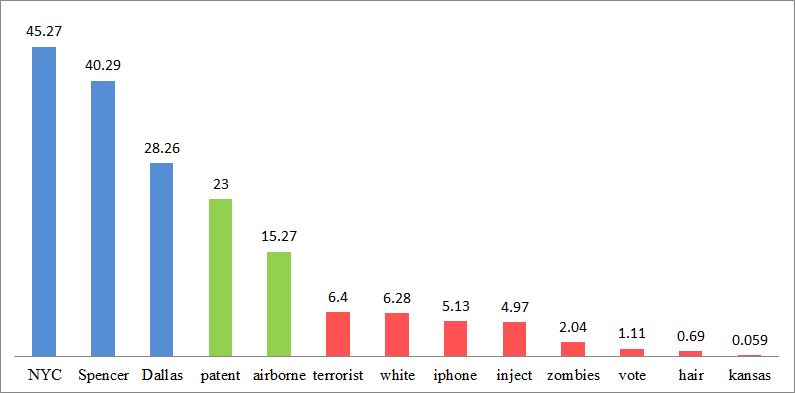
\includegraphics[width=5in]{pictures/Ebola/R_si_values.png} %?????????????
\caption{Ultimate response ratios for 3 news stories (left) and 10 rumors related to Ebola.}
\label{fig:Ebola_response_ratio}
\end{figure}


\begin{figure}[h]
\centering
  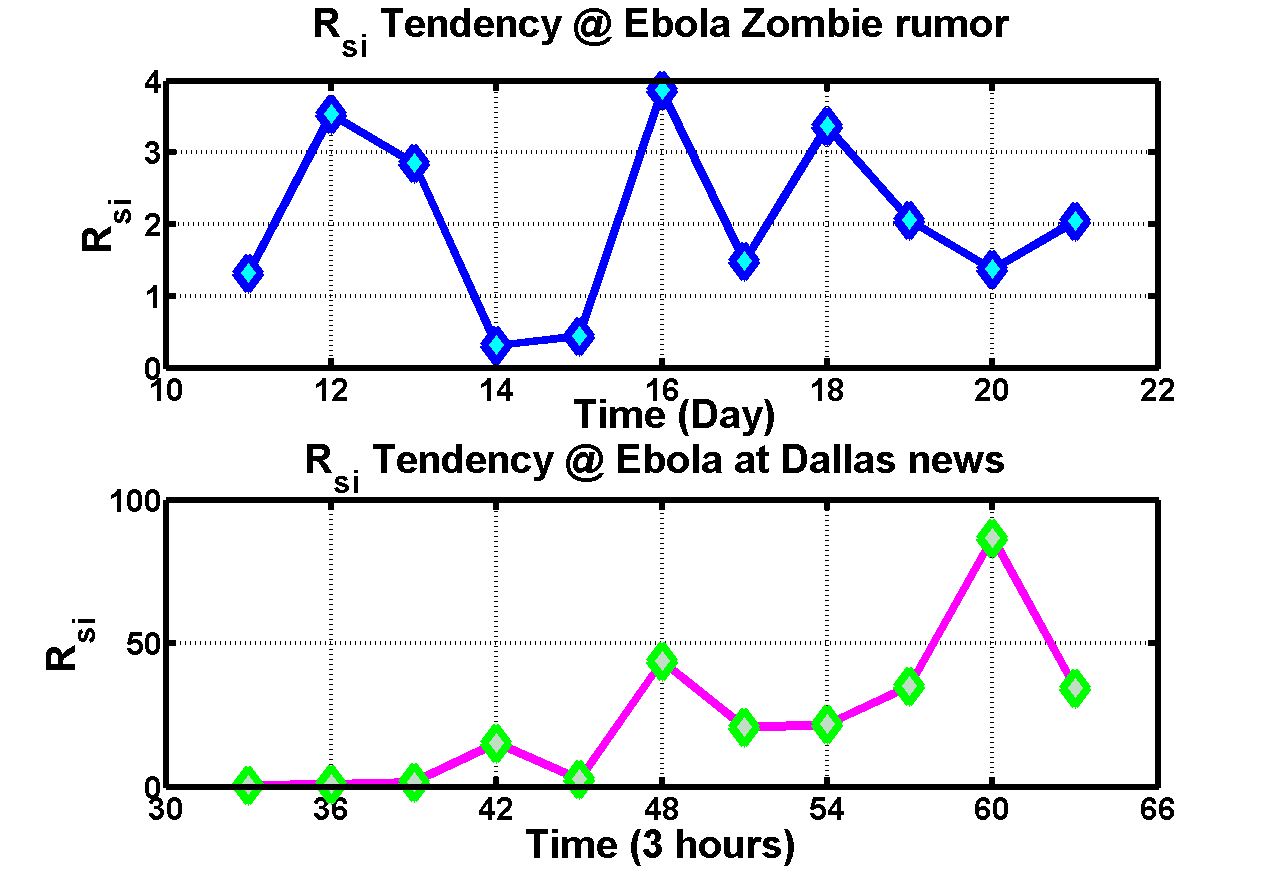
\includegraphics[width=5in]{pictures/Ebola/real-time-RSI-value-Ebloa.png}
   \caption{Dynamic $R_{SI}$ values for Zombie rumor and Dallas real news.}
  \label{fig:dynamic_zombie_ratio}
\end{figure}



\paragraph{Ultimate $R_{SI}$ value}

The ultimate response ratios for these three news stories and other rumors are shown in Figure~\ref{fig:Ebola_response_ratio}. It can be seen that all three news stories (blue bars) have response ratios higher than 25, with a mean value of approximately 38, while eight of the 10 rumors stories (red bars) have a response ratio less than or equal to 6.4, with a mean of only 3.33. Two of the 10 rumors (green bars; `paten' and `airborne') have elevated response values, suggesting that there was greater belief associated with these topics than the other eight rumors.

\paragraph{Dynamic $R_{SI}$ value}
Figure~\ref{fig:dynamic_zombie_ratio} illustrates the dynamic response ratio of Zombie rumor and Dallas real news. We can see the response ratio for Ebola Zombie rumor swings between 0 to 4, which means people's believe extent to Zombie rumor has been very low. However, the dynamic response ratio for Dallas real news kept increasing and reached as high as nearly 100, which reveals more and more people accept this real news.


The study here has shown that propagation of misinformation can sometimes have the same characteristics as genuine newsworthy developments.  In an age where many consumers receive their news from real-time social media platforms, it is imperative that rumors and half-truths be characterized as such and able to be distinguished from news. The tools presented here can support the quantitative evaluation of information spread as it happens.
